\paragraph{Sơ đồ tuần tự luồng tra cứu lịch sử giao dịch}

Luồng nghiệp vụ này mô tả

quy trình User tra cứu danh sách giao dịch thanh toán mua gói thuê bao VIP. Web Frontend gọi Payment Service qua API Gateway, backend truy vấn transaction theo \texttt{userId}, trả về \texttt{BaseResponse} chứa \texttt{items} và \texttt{total}, sau đó Frontend bóc \texttt{data} bằng \texttt{apiHelper}.

\begin{figure}[H]
\centering
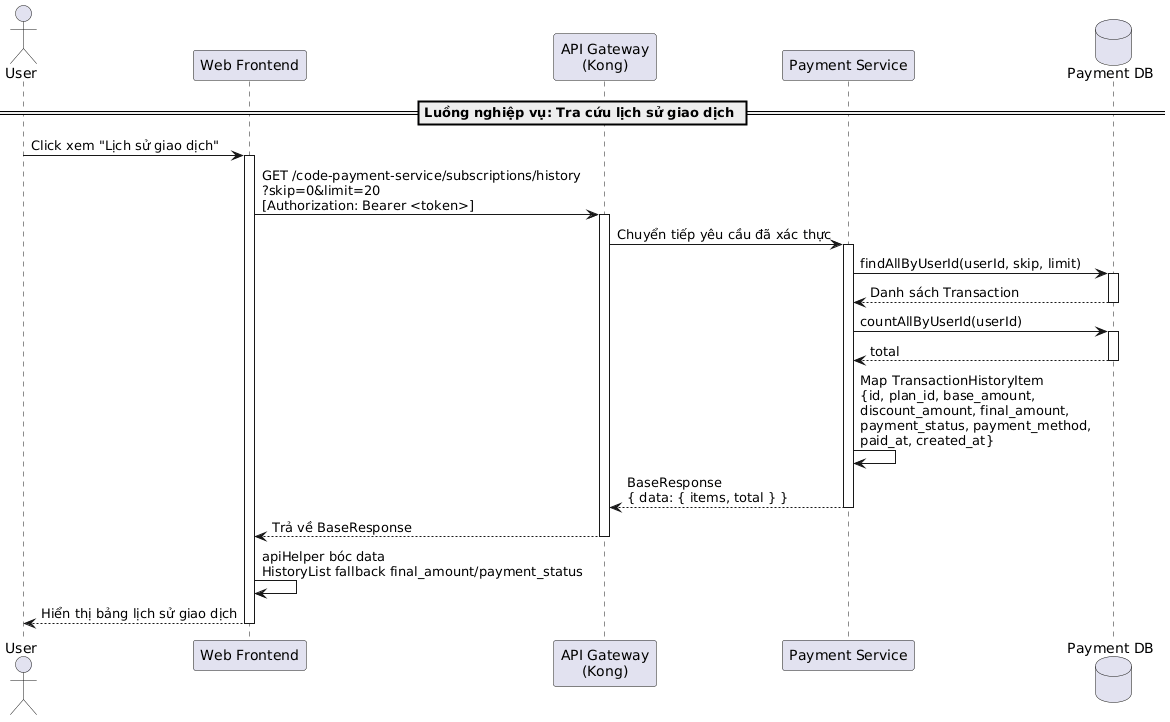
\includegraphics[scale = 0.18]{contents/Sequence/UML-Sequence-UserTransactionHistoryLookup.png}
\caption{Sơ đồ tuần tự luồng tra cứu lịch sử giao dịch}
\end{figure}

\subparagraph{Các thành phần tham gia}

\begin{table}[H]
\centering
\renewcommand{\arraystretch}{1.3}
\begin{tabular}{|l|l|p{5cm}|}
\hline
\textbf{Thành phần} & \textbf{Phân loại} & \textbf{Vai trò trong hệ thống} \\ \hline
User & Actor & Người dùng yêu cầu tra cứu lịch sử giao dịch cá nhân. \\ \hline
Web Frontend & Component & Giao diện web Next.js. \\ \hline %%%% Component & Gọi \texttt{paymentService.getTransactionHistory}, bóc dữ liệu trả về và hiển thị bảng lịch sử. \\ \hline
API Gateway (Kong) & Component & Cổng API chuyển tiếp các yêu cầu API. \\ \hline %%%% Component & Xác thực token người dùng và định tuyến yêu cầu tới Payment Service. \\ \hline
Payment Service & Microservice & Tiếp nhận query, lấy danh sách transaction và tổng số bản ghi theo \texttt{userId}. \\ \hline
Payment DB & Database & Lưu thông tin Transaction của người dùng. \\ \hline
\end{tabular}
\caption{Các thành phần tham gia luồng tra cứu lịch sử giao dịch}
\end{table}

\subparagraph{Mô tả tổng quan}
\begin{itemize}
\item \textbf{Yêu cầu tra cứu:} User mở trang Lịch sử giao dịch. Web Frontend gọi \texttt{GET /code-payment-service/subscriptions/history} với tham số \texttt{skip}, \texttt{limit} và Bearer Token.
\item \textbf{Xử lý truy vấn:} Payment Service tạo \texttt{GetTransactionHistoryQuery}, truy vấn \texttt{findAllByUserId(userId, skip, limit)} để lấy danh sách transaction và \texttt{countAllByUserId(userId)} để lấy \texttt{total}.
\item \textbf{Ánh xạ DTO:} Backend ánh xạ mỗi transaction thành item gồm \texttt{id}, \texttt{plan\_id}, \texttt{base\_amount}, \texttt{discount\_amount}, \texttt{final\_amount}, \texttt{payment\_status}, \texttt{payment\_method}, \texttt{paid\_at}, \texttt{created\_at}.
\item \textbf{Phản hồi dữ liệu:} Payment Service trả \texttt{BaseResponse} với \texttt{data=\{ items, total \}}. Frontend dùng \texttt{apiHelper} bóc \texttt{data}; \texttt{HistoryList} hiển thị số tiền từ \texttt{final\_amount} và trạng thái từ \texttt{payment\_status}.
\end{itemize}
